\def\bmu{{\bs \mu}}
\def\hmu{{\hat{\bs \mu}}}\def\hr{{\hat{\bs r}}}
\problem{20}
The majority of intermolecular interactions originate from electrostatic interactions.
The simplest form is given by the Coulombic energy between 
two point charges ($q_1$ and $q_2$) in a vacuum,
\[ u_{\rm pp} = \frac{1}{4\pi\epsilon_0} \frac{q_1 q_2}{r} .\]
Here $\epsilon_0 = 8.85\times10^{-12}\rm\,F/m$ is the vacuum permittivity,
and $r$ is the distance between $q_1$ and $q_2$.
Although the equation above is simple,
molecules are charge-neutral and can't be
treated as single point charges. 
The dominating electrostatic term is therefore
given by the interaction between electric dipoles.
In this problem, we will derive the separation dependence
of dipole-dipole interactions.

\smallskip \subp
Charge separation within a molecule gives rise to a molecular dipole, $\bmu_1$.
The dipole is a vector pointing from the negative charge center
to the positive charge center, with magnitude equal to
the product of the charge and 
the separation vector (i.e. $\bmu_1 = q \bs d$).
\begin{figure}[h]\centering
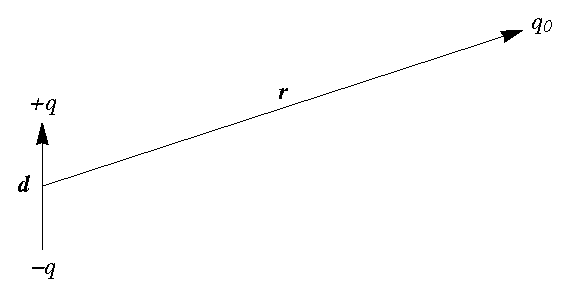
\includegraphics[width=0.4\textwidth,height=!]{dipolepoint}
\end{figure}
Consider first how this dipole interacts 
with a point charge $q_0$ located at $\bs r$.
Show that, when the intra-molecular charge separation $d$ is much
less than the distance $r$,
the total Coulombic potential is given by
$$ u_{\rm dp} = \frac{q_0}{4\pi\epsilon_0} \frac{\bmu_1 \cdot \hat{\bs r}}{r^2} .$$
Above, $\hat{\bs r} \equiv {\bs r} / r$ is a unit vector used to indicate directionality.
Note that $u_{\rm dp}$ decays with $1/r^2$ and 
depends on the orientation of the dipole. 
\solution{\\
{\bf Method I (Geometry): } \\
We need to evaluate the Coulombic energy between
the point charge $q_0$ and the
two dipole partial charges, $+q$ and $-q$.
To do this, we must find $r_+$ and $r_-$
defined in the figure below.
\begin{center}
\includegraphics[width=0.4\textwidth,height=!]{dipolepointsol}
\end{center}
The vector ${\bs r}$ must be defined
with origin at the midpoint between $+q$ and $-q$
(this is the definition of a dipole; 
it is really the only point where it makes sense
to define the distance relative to). 
The angle $\theta$ can be backed out of the dot product:
\[ \cos \theta = \frac{{\bf d}\cdot{\bs r}}{|{\bf d}||{\bs r}|}
               = \frac{\bmu_1 \cdot \hat{\bs r}}{q d} \]
With $\theta$, we can use the law of cosines
to evaluate $r_+$ and $r_-$.
\[ r_+^2 = r^2 + \left( \frac{d}{2} \right)^2 
         - r d \cos \theta 
         = r^2 \left[ 1 + \left( \frac{d}{r} \right)^2 
         - \left(\frac{d}{r} \right) \cos \theta \right] \]
\[ r_-^2 = r^2 + \left( \frac{d}{2} \right)^2 
         - r d \cos \left( \pi - \theta \right) 
         = r^2 \left[ 1 + \left( \frac{d}{r} \right)^2 
         + \left(\frac{d}{r} \right) \cos \theta \right] \]
Assuming $r \gg d$, $(d/r) \ll 1$.
To apply the Coulombic energy between point charges, 
we need $1/r_+$ and $1/r_-$. 
In the large $r$ limit, we can Taylor expand these expressions:
\[ \frac{1}{r_+} \approx \frac{1}{r} \left[1 - (d/r) \cos \theta 
                       + \left( \frac{d}{r} \right)^2 \right]^{-1/2} 
       \approx \frac{1}{r} + \frac{d \cos \theta}{2 r^2} + \ldots \]
\[ \frac{1}{r_-} \approx \frac{1}{r} \left[1 - (d/r) \cos \theta
                       + \left( \frac{d}{r} \right)^2 \right]^{-1/2}
       \approx \frac{1}{r} - \frac{d \cos \theta}{2 r^2} + \ldots \]
The dipole-point interaction can be written as the sum of
two point-point interactions:
\[ u_{\rm dp}  
 = \frac{1}{4 \pi \epsilon_0} 
   \left( \frac{q_0 (q)}{r_+} 
        + \frac{q_0 (-q)}{r_-} \right)
 = \frac{q_0 q}{4 \pi \epsilon_0}
   \left[ \left( \frac{1}{r} + \frac{d \cos \theta}{2r^2} + \ldots \right)
        - \left( \frac{1}{r} - \frac{d \cos \theta}{2r^2} + \ldots \right)
   \right] \]
In the $r \gg d$ limit, we can drop the higher order terms
in the Taylor expansions. Now, we substitute in
the expression for $\cos \theta$ derived above:
\[ \lim_{r \gg d} u_{\rm dp} 
 = \frac{q_0 q}{4 \pi \epsilon_0} 
   \left( \frac{d \cos \theta}{r^2} \right) 
 = \frac{q_0 q}{4 \pi \epsilon_0} 
   \left( \frac{d \bmu_1 \cdot \hat{\bs r}}{r^2 q d} \right)
   \]
Notice that $q$ and $d$ cancel out because they
are wrapped into $\bmu_1$. Thus, when $r \gg d$:
\[ \boxed{ \mu_{\rm dp} = \frac{q_0}{4 \pi \epsilon_0} 
                          \frac{\bmu_1 \cdot \hat{\bs r}}{r^2} } \]
{\bf Method II: } \\
The approach given above, while transparent, 
is a lot of work. 
We would like to evaluate $u_{\rm dp} = -\bmu_1 \cdot {\bf E}_{\rm p}$.
We can do this naturally by noting that $u_{\rm pp} = q_1 V_{\rm p,2}$.
By inspection, $V_{\rm p,2} = \frac{q_2}{4 \pi \epsilon_0 r}$.
Apply this result to the point-dipole case:
\[ {\bf E}_{\rm p} = -\nabla V_{\rm p} 
 = -\nabla \left( \frac{q_0}{4 \pi \epsilon_0 r} \right) 
 = -\frac{q_0}{4 \pi \epsilon_0} \nabla \left( \frac{1}{r} \right) \]
You could evaluate the gradient by imposing
Cartesian coordinates and noting that $r^2 \equiv x^2 + y^2 + z^2$,
but since this is a graduate class (and because you need it for part b),
we will do this with index notation.
\[ \partial_i \left( \frac{1}{r} \right) 
 = \frac{\dd (1/r)}{\dd r} \partial_i r 
 = -\frac{\hat{\bs r}}{r^2} \]
Here, it is understood that $\partial_i r = \hat{\bs r}$.
The vector differential of ${\bs r}$ is simply its direction.
If you prefer rigorous math, note that $r = (r_j r_j)^{1/2}$:
\[ \partial_i (r_j r_j)^{1/2} 
 = \frac{1}{2 (r_k r_k)^{1/2}} \partial_i (r_j r_j) 
 = \frac{1}{2r} \left( 2 r_j \delta_{ij} \right)
 = \frac{r_i}{r} \equiv \hat{\bs r} \]
There is one final complication in evaluating ${\bf E}_{\rm p}$.
The electric field we derived above is for 
a point charge located at the origin;
however, we have selected our dipole as the origin.
Since this is a two-body system, you can convince yourself
that we can correct this by flipping the direction of ${\bs r}$.
Replace $\hat{\bs r}$ with $-\hat{\bs r}$:
\[ {\bf E}_{\rm p} 
 = -\frac{q_0}{4 \pi \epsilon_0} \nabla \left( \frac{1}{r} \right) 
 = -\frac{q_0}{4 \pi \epsilon_0} \left( \frac{\hat{\bs r}}{r^2}\right)
 = -\frac{q_0 \hat{\bs r}}{4 \pi \epsilon_0 r^2}\]
Directly calculate $u_{\rm dp}$.
Remember this is only valid when $r \gg d$.
\[ \boxed{ u_{\rm dp} = -\bmu_1 \cdot {\bf E}_{\rm p} 
 = \frac{q_0}{4\pi \epsilon_0} \frac{\bmu_1 \cdot \hat{\bs r}}{r^2} } \]
}

\smallskip \subp 
Replace the point charge $q_0$ with a second dipole ${\bs \mu}_2$.
Show that, when the separation $r$ is large,
the interaction between these two dipoles is given by
$$ u_{\rm dd} = \frac{1}{4\pi\epsilon_0}
\frac{\bmu_1 \cdot
\left({\bf I} - 3\, \hat{\bs r}\hat{\bs r} \right)
\cdot \bmu_2
}{r^3} .$$
Above $\bf I$ is an isotropic $3\times3$ tensor.
The dyad $\hat{\bs r}\hat{\bs r}$ can be viewed as a $3\times 3$ array,
whose entries are given by the product $\hat{\bs r}_i \hat{\bs r}_j$.
Note that $u_{\rm dd}$ decays with $1/r^3$.
\solution{\\
The best approach is to find the electric field due to a dipole.
Then, $u_{\rm dd} = -\bmu_2 \cdot {\bf E}_{\rm d}$ can be evaluated.
Since $u_{\rm dp} = q_0 V_d$, we use part (a) to write:
\[ {\bf E}_{\rm d} = -\nabla V_d 
 = -\nabla \left( \frac{\bmu_1 \cdot \hat{\bs r}}{4 \pi \epsilon_0 r^2} \right) 
 = -\frac{1}{4 \pi \epsilon_0} \nabla 
    \left( \frac{\bmu_1 \cdot {\bs r}}{r^3} \right) \]
Note that $\bmu_1$ is constant. Using index notation is a good idea
(Remember that $\partial_j r = \hat{\bs r}_j$):
\begin{align*}
   \nabla \left( \frac{\bmu_1 \cdot {\bs r}}{r^3} \right) 
  &\Rightarrow \mu_i \partial_j \left( \frac{r_i}{r^3} \right)
 = \frac{\mu_i}{r^3} \partial_j r_i 
 + \mu_i r_i \partial_j \left( \frac{1}{r^3} \right)
 = \frac{\mu_i \delta_{ij}}{r^3} 
 - \frac{3 \mu_i r_i}{r^4} \partial_j r \\
&= \frac{\mu_i \delta_{ij}}{r^3} 
 - \frac{3 \mu_i \hat{r}_i \hat{r}_j}{r^3}
 = \frac{\mu_i (\delta_{ij} - 3 \hat{r}_i \hat{r}_j)}{r^3}
\end{align*} 
The expression in parenthesis is the index notation representation
of $({\bf I} - 3 \hat{\bs r} \hat{\bs r})$, where the second
term is the dyad of ${\bs r}$. 
Thus, the electric field due to dipole 1 (at the origin) is:
\[ {\bf E}_{\rm d} = \frac{-1}{4 \pi \epsilon_0} 
   \frac{\bmu_1 \cdot ({\bf I} - 3 \hat{\bs r} \hat{\bs r})}{r^3} \]
We are basically done. Again, do not forget
this is only valid when $r \gg d$, such that
the electric field from one dipole is approximately
constant in the vicinity of the other dipole.
\[ \boxed{ u_{\rm dd} = -\bmu_2 \cdot {\bf E}_{\rm d} 
 = \frac{1}{4 \pi \epsilon_0} 
   \frac{\bmu_1 \cdot ({\bf I} - 3 \hat{\bs r} \hat{\bs r}) \cdot \bmu_2}{r^3} } \]
}

\smallskip \subp
The orientation of molecular dipoles changes rapidly 
(recall that the effective temperature for rotational degrees of freedom 
 is $\theta_{\rm rot} \simeq \rm10\,K$).
The effective interaction between molecules
must therefore be averaged over the fluctuating
orientation of the dipoles $\bmu_1$ and $\bmu_2$.
%Denote the average of a quantity $O$ over the molecular orientation by
%$\ave{O} \equiv \frac{1}{4\pi} \int_0^\pi\!\sin\theta\dd\theta \int_0^{2\pi}\!\dd\phi \cdot$.
To find the form of this effective interaction,
start by looking at the summation over Boltzmann factors
for the translational and orientational degrees of freedom for the two molecules:
\begin{align*}
& \int\!\dd{\bf r_1} \!
\int\!\dd{\bf r_2}
\int\!\frac{\dd{{\hat \bmu}_1}}{4\pi} \!
\int\!\frac{\dd{{\hat \bmu}_2}}{4\pi} \,
\exp\left( -\frac{u_{\rm dd}(\bf r_2 - \bf r_1; \bmu_1, \bmu_2)}{\kT} \right)
\equiv  \int\!\dd{\bf r_1} \! \int\!\dd{\bf r_2}
\exp\left( -\frac{w_{\rm dd}(\bf r_2 - \bf r_1)}{\kT} \right) .
\end{align*}
The factor of $4\pi$ is introduced to normalize the
integrals over $\hat{\bmu}_1$ and $\hat{\bmu}_2$.
The effective potential $w_{\rm dd}(\bf r)$ 
encapsulates orientation effects and is defined by
$$
w_{\rm dd}({\bf r}) =
- \kT \ln \left[\int\!\frac{\dd{{\hat \bmu}_1}}{4\pi} \!
\int\!\frac{\dd{{\hat \bmu}_2}}{4\pi} \,
\exp\left( -\frac{u_{\rm dd}(\bf r; \bmu_1, \bmu_2)}{\kT} \right)\right] .
$$
To simplify the notation, let
$\ave{O} \equiv \int\!\frac{\dd{{\hat \bmu}_1}}{4\pi} \!
\int\!\frac{\dd{{\hat \bmu}_2}}{4\pi} \, O $.
Show that, when the potential $u_{\rm dd}$ is small compared to $\kT$,
the effective interaction can be written
$$ w_{\rm dd}({\bf r}) = \ave{u_{\rm dd}} - \frac{1}{2\,\kT}
\left( \ave{u_{\rm dd}^2}  - \ave{u_{\rm dd}}^2 \right) .$$
\solution{\\
Assuming that $u_{\rm dd} \ll \kT$, then we can Taylor expand
the Boltzmann factor:
\[ \exp \left(- \frac{u_{\rm dd}}{\kT} \right) 
   \approx 1 - \frac{u_{\rm dd}}{\kT} 
 + \frac{1}{2} \left( \frac{u_{\rm dd}}{\kT} \right)^2 + \ldots \]
Apply the definition of $\ave{O}$:
\[ w_{\rm dd} ({\bf r}) = -\kT \ln 
  \left[ \ave{1} - \frac{\ave{u_{\rm dd}}}{\kT} 
       + \frac{\ave{u_{\rm dd}^2}}{2 (\kT)^2} + \ldots \right] \]
Since $\ave{1} = 1$, Taylor expand the logarithm too:
\[ \ln \left[ 1 - \frac{\ave{u_{\rm dd}}}{\kT} 
            + \frac{\ave{u_{\rm dd}^2}}{2 (\kT)^2} + \ldots \right] 
 \approx    - \left[ \frac{\ave{u_{\rm dd}}}{\kT} 
            - \frac{\ave{u_{\rm dd}^2}}{2 (\kT)^2} \right] 
 -\frac{1}{2} \left[ \frac{\ave{u_{\rm dd}}}{\kT} 
            - \frac{\ave{u_{\rm dd}^2}}{2 (\kT)^2} \right]^2 + \ldots \]
Keep up to second order terms:
\[ \ln \left[ 1 - \frac{\ave{u_{\rm dd}}}{\kT} 
            + \frac{\ave{u_{\rm dd}^2}}{2 (\kT)^2} + \ldots \right] 
    \approx - \frac{\ave{u_{\rm dd}}}{\kT} 
            + \frac{\ave{u_{\rm dd}^2}}{2 (\kT)^2} 
            - \frac{\ave{u_{\rm dd}}^2}{2 (\kT)^2} + \ldots \]
Multiply by $-\kT$ and do a little bit of rearranging to get:
\[ \boxed{ w_{\rm dd} ({\vec r}) = \ave{u_{\rm dd}} - \frac{1}{2\,\kT}
   \left( \ave{u_{\rm dd}^2}  - \ave{u_{\rm dd}}^2 \right) } \]
}

\smallskip \subp
For the specific form of the dipole-dipole interaction
derived in (b),
show that $\ave{u_{\rm dd}} = 0$ and
$$ w_{\rm dd}({\bs r}) = - \left[\frac{1}{3\,\kT}
\frac{\mu_1^2 \mu_2^2}{(4\pi\epsilon_0)^2}\right] \frac{1}{r^6} .$$
This potential is known as the Keesom interaction.
It is attractive, decays as $r^{-6}$,
and is one of the three potentials that
comprise the Van~der~Waals interaction.
The other two potentials are related to
interactions between dipoles and induced dipoles,
and also scale with $r^{-6}$.
%The induced dipole is proportional to field strength which scales as $r^{-3}$,
%and the dipole-dipole interaction contributes another factor $r^{-3}$.
%As a result, they also decay as $r^{-6}$.
\solution{ \\
Begin by evaluating $\ave{u_{\rm dd}}$. 
The non-bold $\mu_1 \equiv |\bmu_1|$
is the magnitude of the dipole moment.
\[ u_{\rm dd} = \frac{1}{4 \pi \epsilon_0} 
   \frac{\bmu_1 \cdot ({\bf I} - 3 \hat{\bs r} \hat{\bs r}) \cdot \bmu_2}{r^3} 
 = \frac{\mu_1 \mu_2}{4 \pi \epsilon_0 r^3} 
   \left[ \hmu_1 \cdot \hmu_2 
        - 3(\hmu_1 \cdot \hat{\bs r})(\hmu_2 \cdot \hat{\bs r}) \right] \]
In the following, we will keep the notation simple
by using angle-brackets as a shorthand
for the orientational average integrals 
$\int \frac{\dd \hmu_1}{4\pi}$ and $\int \frac{\dd \hmu_2}{4\pi}$.
\[ \ave{u_{\rm dd}} = \frac{\mu_1 \mu_2}{4 \pi \epsilon_0 r^3}  
   \left[ \ave{\hmu_1} \cdot \ave{\hmu_2} 
     - 3 (\ave{\hmu_1}\cdot \hr )(\ave{\hmu_2} \cdot \hr) \right] \]
Above, $\hr$ is constant with respect to the orientation average,
and we can split the averages up because integration over
$\hmu_1$ and $\hmu_2$ is independent.\\ \\
We need not evaluate $\ave{\hmu_1}$ 
to know that it is zero.
This integral $\int \dd \hmu_1$ is the same as
integrating over all possible unit vectors from the origin 
to the surface of a unit sphere.
Thus, $\ave{\hmu_1} = \int \frac{\dd \hmu_1}{4\pi}\,\hmu_1$
is zero, since every possible orientation has an opposite.
\[ \ave{u_{\rm dd}} = \frac{\mu_1 \mu_2}{4 \pi \epsilon_0 r^3}  
   \left[ 0 - 0 \right]  = 0 \]
Now that we've shown $\ave{u_{\rm dd}} = 0$, let us
impose the additional constraint that $u_{\rm dd} \ll \kT$.
We can use the result of part (c) to write the expression:
\[ w_{\rm dd} ({\bs r}) = - \frac{\ave{u_{\rm dd}^2}}{2\kT} \]
The problem reduces to evaluating $\ave{u_{\rm dd}^2}$.
\[ u_{\rm dd}^2 = \left( \frac{\mu_1 \mu_2}{4 \pi \epsilon_0 r^3} \right)^2
   \left[ \left( \hmu_1 \cdot \hmu_2 \right)^2
        - 6 \hr \cdot \hmu_1 \hmu_1 \cdot \hmu_2 \hmu_2 \cdot \hr 
        + 9 (\hmu_1 \cdot \hat{\bs r})^2(\hmu_2 \cdot \hat{\bs r})^2 \right] \]
The quantities $\hmu_1 \hmu_1$ and $\hmu_2 \hmu_2$ are dyadic products 
(try index notation if you don't understand how to pull 
these out of the expression).
Let the kernel $K^2$ denote the quantity in brackets.
The leading factor does not have orientation dependence,
so our problem is really just evaluating 
the orientation average of $K^2$.
\begin{align*}
\ave{K^2} &= \ave{(\hmu_1\cdot\hmu_2)^2} -
6 \hr\cdot\ave{\hmu_1\hmu_1}\cdot
  \ave{\hmu_2\hmu_2}\cdot \hr +
9 \ave{(\hmu_1\cdot \hr)^2} \ave{(\hr \cdot \hmu_2)^2}
\end{align*}
To get the first term, integrate 
over $\hmu_1$ and $\hmu_2$ separately -- 
that is, fix $\hmu_1$ to be the $+z$ direction
and switch the other integral to spherical coordinates.
\begin{align*}
    \ave{(\hmu_1\cdot\hmu_2)^2} 
 &= \int \frac{\dd \hmu_1}{4\pi} \int \frac{\dd \hmu_2}{4\pi} \,
    (\hmu_1 \cdot \hmu_2)^2
  = \int \frac{\dd \hmu_1}{4\pi} \frac{1}{4\pi} 
    \left[ \int_0^{2\pi} \dd \phi \int_0^{\pi} \dd \theta \, 
           (\cos \theta)^2 \sin \theta \right]  \\
 &= \int \frac{\dd \hmu_1}{4\pi} \frac{ (2\pi) (2/3) }{4\pi} 
  = \int \frac{\dd \hmu_1}{4\pi} \left( \frac{1}{3} \right) = \frac{1}{3}
\end{align*}
To get the second term, notice that
$\ave{\hmu_1\hmu_1} = \ave{\hmu_2\hmu_2} = \int \frac{\dd \hmu}{4\pi} (\hmu \hmu)$.
The result is a second-order tensor, and must be 
isotropic because the orientation average integral
must be invariant with respect to rotation.
Since ${\bf Tr} (\hmu \hmu) = \hmu \cdot \hmu = 1$,
$\ave{\hmu \hmu} = (1/3){\bf I}$ 
(recall ${\bf I} = \delta_{ij}$ is the only isotropic second-order tensor).
The second term is best evaluated in index notation:
\[ 6 \hr\cdot\ave{\hmu_1\hmu_1}\cdot \ave{\hmu_2\hmu_2}\cdot \hr 
 = 6 \hat{r}_i \frac{\delta_{ij}}{3} \frac{\delta_{jk}}{3} \hat{r}_k 
 = \frac{2}{3} \hat{r}_i \hat{r}_i = \frac{2}{3} \]
The third term is the same integration
as the first term (one vector is changing orientation,
the other one is fixed), so each dot product squared 
averages to $1/3$.
\[ 9 \ave{(\hmu_1\cdot \hr)^2} \ave{(\hr \cdot \hmu_2)^2} 
 = 9 \left( \frac{1}{3} \right) \left( \frac{1}{3} \right) = 1 \]
\iffalse
Alternatively, you do the following:
\begin{align*}
\ave{K^2} &=
\ave{(\hmu_1\cdot\hmu_2)^2} -
6 \hr\cdot\ave{\hmu_1\hmu_1}\cdot
  \ave{\hmu_2\hmu_2}\cdot \hr +
9 \ave{(\hmu_1\cdot \hr)^2} \ave{(\hr \cdot \hmu_2)^2} \\
& = \ave{\hmu_2\cdot
    \ave{\hmu_1\hmu_1}_1\cdot\hmu_2}_2 -
6 \hr\cdot\ave{\hmu_1\hmu_1}\cdot
  \ave{\hmu_2\hmu_2}\cdot \hr +
9 \hr\cdot\ave{\hmu_1\hmu_1}_1\cdot\hr\hr\cdot
  \ave{\hmu_2\hmu_2}_2\cdot\hr
 = \frac{2}{3}.
\end{align*}
\fi
Thus, we have shown that:
\[ \ave{K^2} = \frac{1}{3} - \frac{2}{3} + 1 = \frac{2}{3} \]
\[ \ave{u_{\rm dd}^2} 
= \left( \frac{\mu_1 \mu_2}{4 \pi \epsilon_0 r^3} \right)^2 \ave{K^2} 
= \frac{2}{3} \left( \frac{\mu_1 \mu_2}{4 \pi \epsilon_0 r^3} \right)^2 \]
Plug back into the equation we derived in (c) to get:
\[ w_{\rm dd} ({\bs r}) = \frac{-1}{3 \kT}
   \left( \frac{\mu_1 \mu_2}{4 \pi \epsilon_0 r^3} \right)^2 \]
This is precisely what we wanted to show.
\[  \boxed{ w_{\rm dd} ({\bs r}) 
 = -\left[ \frac{1}{3\kT} \frac{\mu_1^2 \mu_2^2}{(4 \pi \epsilon_0)^2} \right] 
    \frac{1}{r^6} } \]
\newpage}

\bigskip
\problem{30}
Consider a system of $N$ molecules that are covalently bonded to a surface.
The surface coverage is sufficiently small such
that we can consider the molecules to be non-interacting.
These flexible molecules have favorable surface interactions
and prefer to lie down on the surface.   
Let us apply the following simplified model.
Suppose each molecule consists of four `beads'
connected by 3 bonds (see Fig.~\ref{fig:model}), 
and that each bond can orient in one of six possible directions 
($\hat{x}, -\hat{x}, \hat{y}, -\hat{y}, \hat{z}$, or $-\hat{z}$).
The first bead is fixed to the surface, 
and the first bond is pointed away from the surface
in the  $\hat{z}$ direction.  
The other bonds can orient in any of 6 directions subject to the constraint
that no beads can overlap and that no beads (other than the first) can touch the
surface. Each bead that lies next to the surface has a 
favorable interaction energy of $-\epsilon_{0}$.

\begin{figure}[h]\centering
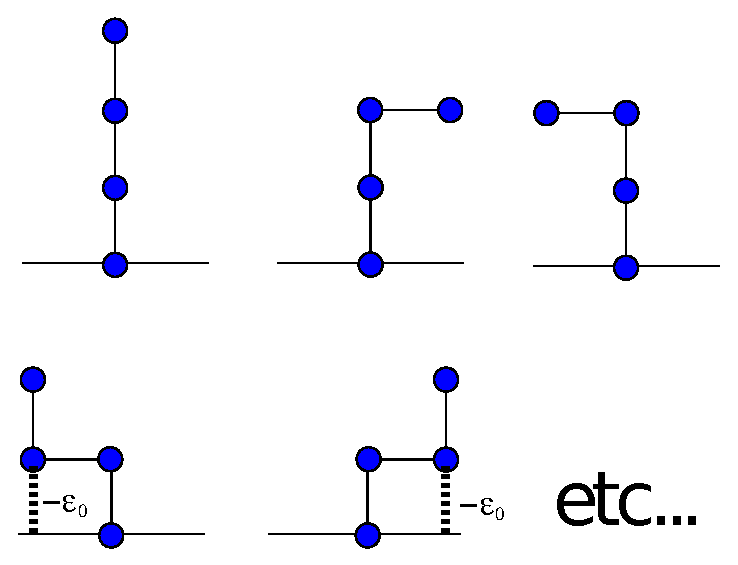
\includegraphics[width=0.35\textwidth,height=!]{molsurf}\par
\bigskip
\caption{
Several configurations of our model for a flexible molecule 
covalently linked to a surface.
The top row shows 3 configurations that have no favorable surface interactions.
The bottom row shows 2 configurations that have 1 favorable surface interaction.
These configurations are only a subset of all possible configurations
with 0, 1, or 2 surface interactions.
\label{fig:model}}
\end{figure}

\smallskip\subp
Find the degeneracies for the states with 
0 surface interactions ($g_{0}$),
1 surface interaction ($g_{1}$),
and 2 surface interactions ($g_{2}$).
\solution{\\
The two beads closest to the surface are always in the same position.
Only beads three and four can take different contributions. 
Bead 3 can be in five locations (all except $-\hat{z}$).
If the bond 2-3 is parallel to the surface, 
then bead four can be in four positions (can't double back, and can't touch the surface). 
If bond 2-3 is perpendicular to the surface, 
bead four can be in one of five positions (can't double back). 
Therefore, there are:
\[ 1*(5) + 4*(4) = 21 \text{ total states} \]
There are five states with no surface interactions
(bead three is $+\hat{z}$ relative to bead 2).
There are four states with only one surface interaction
(bead three is {\bf not} $+\hat{z}$, and bead 4 is $+\hat{z}$).
This leaves $21 - (4 + 5) = 12$ states with two surface interactions.
\[ \boxed{ g_0 = 5 \quad , \quad 
           g_1 = 4 \quad , \quad 
           g_2 = 12 } \]
}

\smallskip\subp
Solve for the single-molecule partition function $q$ 
and the partition function $Q$ for this system using
the degeneracies and the appropriate Boltzmann weights.
Because the molecules are bound to unique surface sites,
you should assume that they are {\bf distinguishable}.
\solution{\\
We use the canonical (N,V,T) ensemble. The single-molecule partition function is:
\[ q = \sum_k \exp \left( \frac{-\epsilon_k}{\kT} \right) 
     = \sum_{n = 0}^2 g_n \exp \left( \frac{-n \varepsilon_0}{\kT} \right) 
     = 5 + 4 \exp \left( \frac{ \varepsilon_0}{\kT} \right) 
         + 12 \exp \left( \frac{2 \varepsilon_0}{\kT} \right) \]
Above, $k$ denotes a `state' (i.e. specific configuration)
and $n$ denotes different energy states ($n$ is the number of surface interactions).
Since the particles are non-interacting and distinguishable,
the partition function for the system of $N$ molecules is simply $Q = q^N$.
\[ \boxed{ Q = q^N = \left[ 5 + 4 \exp \left( \frac{\varepsilon_0}{\kT} \right) 
             + 12 \exp \left( \frac{2 \varepsilon_0}{\kT} \right) \right]^N } \]
}

\smallskip\subp
Find the Helmholtz free energy, the average energy $\left< E \right>$,
and the entropy $S$ of the system of $N$ molecules. 
\solution{\\
The partition function $Q(N,V,T)$ allows us to evaluate thermodynamic quantities:
\begin{align*}
    F &= -\kT \ln Q = -\kT \ln (q^N)
       = -N \kT \ln \left[ 5 + 4 \exp \left( \frac{\varepsilon_0}{\kT} \right) 
       + 12 \exp \left( \frac{2 \varepsilon_0}{\kT} \right) \right] 
\end{align*}
Entropy is a bit messy but only because the expression is large:
\begin{align*}
    S &=  -\pdc{F}{T}{{V,N}} \\
      &= N k_B \ln \left[ 5 + 4 \exp \left( \frac{\varepsilon_0}{\kT} \right) 
       + 12 \exp \left( \frac{2 \varepsilon_0}{\kT} \right) \right] 
       + N \kT \left[ \frac{0 - \frac{4 \varepsilon_0}{\kT^2} 
         \exp \left( \frac{\varepsilon_0}{\kT} \right) - \frac{24 \varepsilon_0}{\kT^2} 
         \exp \left( \frac{2 \varepsilon_0}{\kT} \right) }{5 + 4 
         \exp \left( \frac{\varepsilon_0}{\kT} \right) + 12 
         \exp \left( \frac{2 \varepsilon_0}{\kT} \right) } \right] \\ 
      &= N k_B \left[ \ln \left[ 5 + 4 \exp \left( \frac{\varepsilon_0}{\kT} \right) 
       + 12 \exp \left( \frac{2 \varepsilon_0}{\kT} \right) \right] 
       - \frac{\varepsilon_0}{\kT} \frac{ 4 \exp \left( \frac{\varepsilon_0}{\kT} \right)
       + 24 \exp \left( \frac{2 \varepsilon_0}{\kT} \right) }
         {5 + 4 \exp \left( \frac{\varepsilon_0}{\kT} \right) 
       + 12 \exp \left( \frac{2 \varepsilon_0}{\kT} \right) } \right]
\end{align*}
Remember that the classical $U$ is just $\ave{E}$. 
The first term in entropy (above) is just $-F/T$. 
\begin{align*}
   U &\equiv \ave{E}
     = F + TS 
     = N \kT \left[ - \frac{\varepsilon_0}{\kT} 
       \frac{ 4 \exp \left( \frac{\varepsilon_0}{\kT} \right) 
     + 24 \exp \left( \frac{2 \varepsilon_0}{\kT} \right) }
       {5 + 4 \exp \left( \frac{\varepsilon_0}{\kT} \right) 
     + 12 \exp \left( \frac{2 \varepsilon_0}{\kT} \right) } \right] \\
    &= -N \varepsilon_0 \left[ \frac{ 4 \exp \left( \frac{\varepsilon_0}{\kT} \right) 
     + 24 \exp \left( \frac{2 \varepsilon_0}{\kT} \right) }
       {5 + 4 \exp \left( \frac{\varepsilon_0}{\kT} \right) 
     + 12 \exp \left( \frac{2 \varepsilon_0}{\kT} \right) } \right] 
\end{align*} 
You should be able to see, by inspection, that this is the
literal definition of $\ave{E}$. 
To summarize:
\[ \boxed{ F = -\kT \ln (q^N) 
             = -N \kT \ln \left[ 5 + 4 \exp \left( \frac{\varepsilon_0}{\kT} \right) 
             + 12 \exp \left( \frac{2 \varepsilon_0}{\kT} \right) \right]  } \]
\[ \boxed{ \ave{E} = -N \varepsilon_0 \left[ \frac{ 4 \exp \left( \frac{\varepsilon_0}{\kT} \right) + 24 \exp \left( \frac{2 \varepsilon_0}{\kT} \right) }{5 + 4 \exp \left( \frac{\varepsilon_0}{\kT} \right) + 12 \exp \left( \frac{2 \varepsilon_0}{\kT} \right) } \right] } \]
\[ \boxed{ S = N k_B \left[ \ln \left[ 5 + 4 \exp \left( \frac{\varepsilon_0}{\kT} \right) 
             + 12 \exp \left( \frac{2 \varepsilon_0}{\kT} \right) \right] 
             - \frac{\varepsilon_0}{\kT} \frac{ 4 \exp \left( \frac{\varepsilon_0}{\kT} \right)
             + 24 \exp \left( \frac{2 \varepsilon_0}{\kT} \right) }
               {5 + 4 \exp \left( \frac{\varepsilon_0}{\kT} \right) 
             + 12 \exp \left( \frac{2 \varepsilon_0}{\kT} \right) } \right]} \]
\newpage
}


\smallskip\subp
Evaluate the limit of the average energy $\left< E \right>$
and the entropy $S$ as $T \rightarrow 0$.
\solution{\\
In the limit that $T \rightarrow 0$, the largest exponential terms dominate:
\begin{align*}
   \ave{E} &\approx -N \varepsilon_0 \left[ \frac{0 + 24}{0 + 0 + 12} \right] 
                  = -2 N \varepsilon_0 
\end{align*} \\
Again, the largest exponential terms dominate:
\begin{align*}
    S &\approx N k_B \left[ 
              \ln \left(0+0+12 \exp \left( \frac{2 \varepsilon_0}{\kT} \right) \right)
            - \frac{\varepsilon_0}{\kT} 
              \left( \frac{0+24}{0+0+12} \right) \right] \\
            &= N k_B \left[ \ln(12) + \frac{2\varepsilon_0}{\kT} 
             - \frac{2 \varepsilon_0}{\kT} \right] \\
            &= N k_B \ln (12) 
\end{align*}
Thus, we have found that:
\[ \boxed{ \lim_{T \rightarrow 0} S = N k_B \ln(12) } \]
\[ \boxed{ \lim_{T \rightarrow 0} \ave{E} = -2N\varepsilon_0 } \]
}


\smallskip\subp
Evaluate the limit of the average energy $\left< E \right>$
and the entropy $S$ as $T \rightarrow \infty$.
\solution{\\
In the limit that $T \rightarrow \infty$, the exponentials go to unity.
\[ \ave{E} \approx -N \varepsilon_0 \left[ \frac{4 + 24}{5 + 4 + 12} \right] 
         = -\frac{28}{21} N \varepsilon_0 \]
\[ S \approx N k_B \left[ \ln ( 5 + 4 + 12) - \frac{\varepsilon_0}{\kT} 
     \left( \frac{4 + 24}{5 + 4 + 12} \right) \right] 
   = N k_B \left[ \ln (21) - 0 \right] \] 
We have found the limits:
\[ \boxed{ \lim_{T \rightarrow \infty} S = N k_B \ln(21) } \]
\[ \boxed{ \lim_{T \rightarrow \infty} \ave{E} = -\frac{28}{21} N \varepsilon_0 } \]
}


\smallskip\subp
Plot and explain how the average molecular height will change with temperature.
\solution{
\begin{center}
\includegraphics[width=0.42\textwidth,height=!]{adsorbplot.pdf}
\end{center}
Average molecular height is proportional to $\ave{E}$
because the only energetic term is the favorable surface interaction. 
Therefore, as we increase the temperature of the system, 
the average molecular height will increase 
(energetic differences become unimportant). 
One interesting note: since this is a finite state system,
the temperature is discontinuous and can become negative.
Nevertheless, the statement above is still true.
This is graphically resolved by plotting $\ave{E}$ over $\beta \equiv 1/\kT$:
}
    
    
    
\iffalse
\bigskip
\problem{12}
A plasma or ionized gas may be viewed as a mixture of positive and negative charges.
We consider as our model system a 2-D plasma
(This also happens to be an appropriate model for the motion of
parallel line vortices in an incompressible non-viscous fluid).
A simplified model for 2-D plasma contains
$N$ positive particles with charge density $e_i=e$
and $N$ negative particles with charge density $e_i = -e$ confined in a
two-dimensional ``volume'' $V$. The interaction energy for a given configuration is
$ H = -2\sum_{i<j} e_i e_j K_0\left[a ({\bf r}_i - {\bf r}_j)\right] ,$
where $K_0$ is the Bessel function of imaginary argument
and $a^{-1}$ is a cutoff distance.
By applying a rather ingenious trick, Edwards and Taylor (1974) were able to
obtain an explicit expression for the micro-canonical ensemble
partition function for this model.
Their result reads
$$ \Omega(N, V, U) = \frac{(Va^2)^{2N}}{(2N)!} \int_{-\infty}^{\infty} 
\exp\left[\frac{Va^2}{4\pi} \Big(\img z\epsilon + (1+\img z)\ln(1 + \img z) - \img z\Big) \right] {\rm d}z\,,$$
where $\epsilon \equiv U/(Ne^2)$ and $z$ are dimensionless,
and $\img$ is the imaginary unit.
Note, for this system, it is possible that $U$ is negative,
since two oppositely charged particle in close contact may contribute
a large negative value to the energy.

\smallskip\subp
In the thermodynamic limit, $V \to \infty$,
the partition function is dominated by the saddle point in the integrand.
Apply the steepest descent method, find the saddle point $z^*$,
and compute the partition by using the contribution from the saddle point alone.

\smallskip\subp
Compute the entropy $S(N,V,U)$ using the partition function.
Show that your result is thermodynamically admissible:
entropy $S$ (i) is extensive,
(ii) is a convex function of volume $V$,
and (iii) is a convex function of energy $U$.
Note: convexity $=$ negative curvature.

\smallskip\subp
Derive the equation of state for pressure, i.e., find $P=P(N,V,T)$.

\smallskip\subp
Write down an expression for the inverse temperature $1/T$.
What unusual behavior of temperature can be identified for $U > U_m = 0$?
What is the range of temperatures, for $-\infty < U < \infty$?
Plot the energetic contribution to entropy,
$$ \frac{1}{Va^2 \kB} \left[S - 2N\kB \ln\left(\frac{Va^2\ee}{2N}\right)\right], $$
against $\epsilon=U/(Ne^2)$ for $-1 < \epsilon < 1$.
\hfil\break
\strut\hfil\break
{\sl {\bf FYI:} The unusual behavior arises because the phase space is
bounded for 2-D plasmas and for vortex fluids,
and was first noted by Onsager in 1949
in a famous study of statistical theory on turbulent flow.
It can be visualized by using computer simulations (Fig.~\ref{fig:plasma}) which,
under proper condition, lead to spatial aggregation of particles with equal-sign charges.
The critical energy scale $U_m$ is $-0.4 Ne^2$ for the true plasmas,
which has no long-wavelength cutoff $a^{-1}$.
}

\begin{figure}[h]\centering
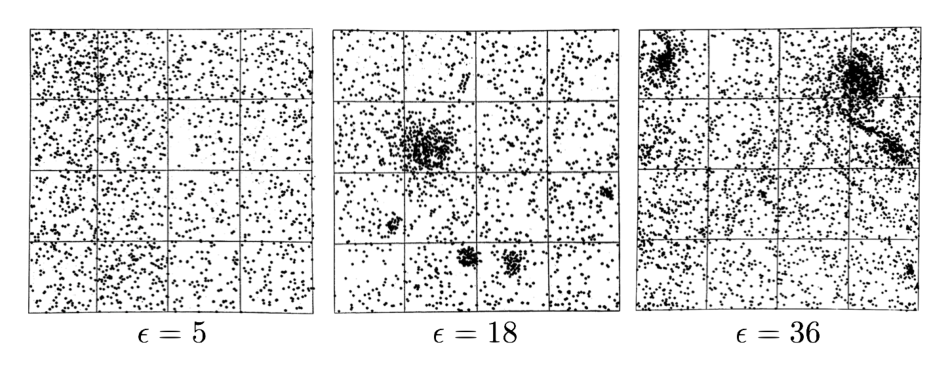
\includegraphics[width=0.618\textwidth,height=!]{plasma}
\caption{
Simulation snapshots for two dimensional plasmas.
Only positive charges are shown.
\label{fig:plasma}}
\end{figure}
\fi
